\documentclass[journal]{IEEEtran}

\usepackage{enumerate}
\usepackage[binary-units=true]{siunitx}
\usepackage{amsfonts,amssymb,amsmath}
\DeclareMathOperator{\Tr}{Tr}

\usepackage{bm,bbm}
\usepackage{subfigure}
\usepackage{array}
\usepackage{breqn}

\DeclareMathOperator*{\argmax}{\arg\!\max}

\usepackage{booktabs}

\usepackage[export]{adjustbox}
\usepackage{multirow}
\usepackage{color}
\usepackage[noabbrev]{cleveref}
\usepackage{cite}

\usepackage{times}
\usepackage{multicol}
\usepackage{graphicx}
\graphicspath{{../../Images/PNG/}{../../Images/PDF/}{../../Plots/PDF/}}

\begin{document}
	
\title{Road Detection from SAR Images with Deep Learning using Simulated Data}
	
\author{Xiangrong Zhang,~\IEEEmembership{Senior Member,~IEEE,}~Zhu Xiao Qian~\IEEEmembership{Student Member,~IEEE,},~and~Alejandro~C.~Frery,~\IEEEmembership{Senior Member,~IEEE}%
	\thanks{X.~Zhang and Z.X. Qian are with the  (e-mail: xrzhang@mail.xidian.edu.cn)}% 
	\thanks{Alejandro~C.~Frery is with the Laborat\'orio de Computa\c c\~ao Cient\'ifica e An\'alise Num\'erica, Universidade Federal de Alagoas, Macei\'o, Brazil, and with the Key Lab of Intelligent Perception and Image Understanding of the Ministry of Education, Xidian University, Xi'an, China.. (e-mail: acfrery@laccan.ufal.br)}% <-this % stops a space
	\thanks{Manuscript received XXX, 2019; revised YYY, 2019.}
	}

\IEEEtitleabstractindextext{%
\begin{abstract}
About NN\dots
We use samples from the Potts model\dots
\end{abstract}

\begin{IEEEkeywords}
SAR, 
speckle, 
simulation, 
\dots
\end{IEEEkeywords}}

\maketitle

\IEEEdisplaynontitleabstractindextext
\IEEEpeerreviewmaketitle

\section{The Sampling Methodology}\label{sec:SamplingMethodology}

We are able to simulate an arbitrary number of samples using a road map.

Consider the model for image formation proposed by Geman and Geman~\cite{geman84}, and later extended by Bustos and Frery~\cite{buseucam92}.
This model states that the observed image $Z$ is the result of a transformation of the unobserved truth $X$.
The transformation consists of:
$\phi$, a possibly nonlinear pointwise transformation of the truth;
$H$, a local degradation of $\phi(X)$;
$Y$, the noise in the form of a random field, that enters the model by pointwise operations $\odot$.
With this, we have:
\begin{equation}
Z = H(\phi(X)) \odot Y.
\label{eq:GemanGeman}
\end{equation}

We propose a pointwise degradation $\phi$ which depends on a random field $X'$.
The local operator $H$ may include problems as occlusions and loss of resolution, but we will not consider it in this work.
With these two considerations, \eqref{eq:GemanGeman} becomes:
\begin{equation}
Z = \phi(X,X') \odot Y.
\label{eq:OurModel}
\end{equation}

Our truth is a map of roads, as illustrated in Fig.~\ref{image:Roads}, which we want to retrieve from a SAR image of the scene.
Figs.~\ref{image:SingleLook} and~\ref{image:ThreeLooks} illustrate two simulated observed SAR images of the scene whose truth is the map of roads.

The truth is transformed in two stages.
The first consists in producing an intermediate truth by ``mixing'' $X$ with a sample from the Potts model $X'$.
The Potts model has a known number of classes $k$, is defined on a grid the same size of $X$, and its inverse temperature parameter is $\beta=\log(1+k^{1/2})$.
Assume the classes are denoted by $\{1,2,\dots,k\}$
Any $\beta$ could be used, but this is the critical value which yields nontrivial patches of classes with high probability.
Winkler~\cite{Winkler2006} provides details about the use of the Potts model in image analysis.
We use the Swendsen-Wang algorithm~\cite{SwendsenWang87} for sampling from this model.
If we denote $X(s)=k+1$ the presence of a road, and $X(s)=0$ otherwise, then the mixing of $X$ and $X'$ can be formulated as
$$
\phi(X) (s)= \left\{
	\begin{array}{cl}
	X'(s)	& \text{if } X(s) = 0,\\
	X(s)	& \text{otherwise.}
	\end{array}
\right.
$$

With this, $\phi(X,X')$ is a map of $k+1$ ordered classes: the first $k$ are the map of the background, and the last one is our class of interest: road.
Notice that it is trivial to define more types of roads.

\begin{figure*}[hbt]
\centering
\subfigure[First map of $5$ classes]{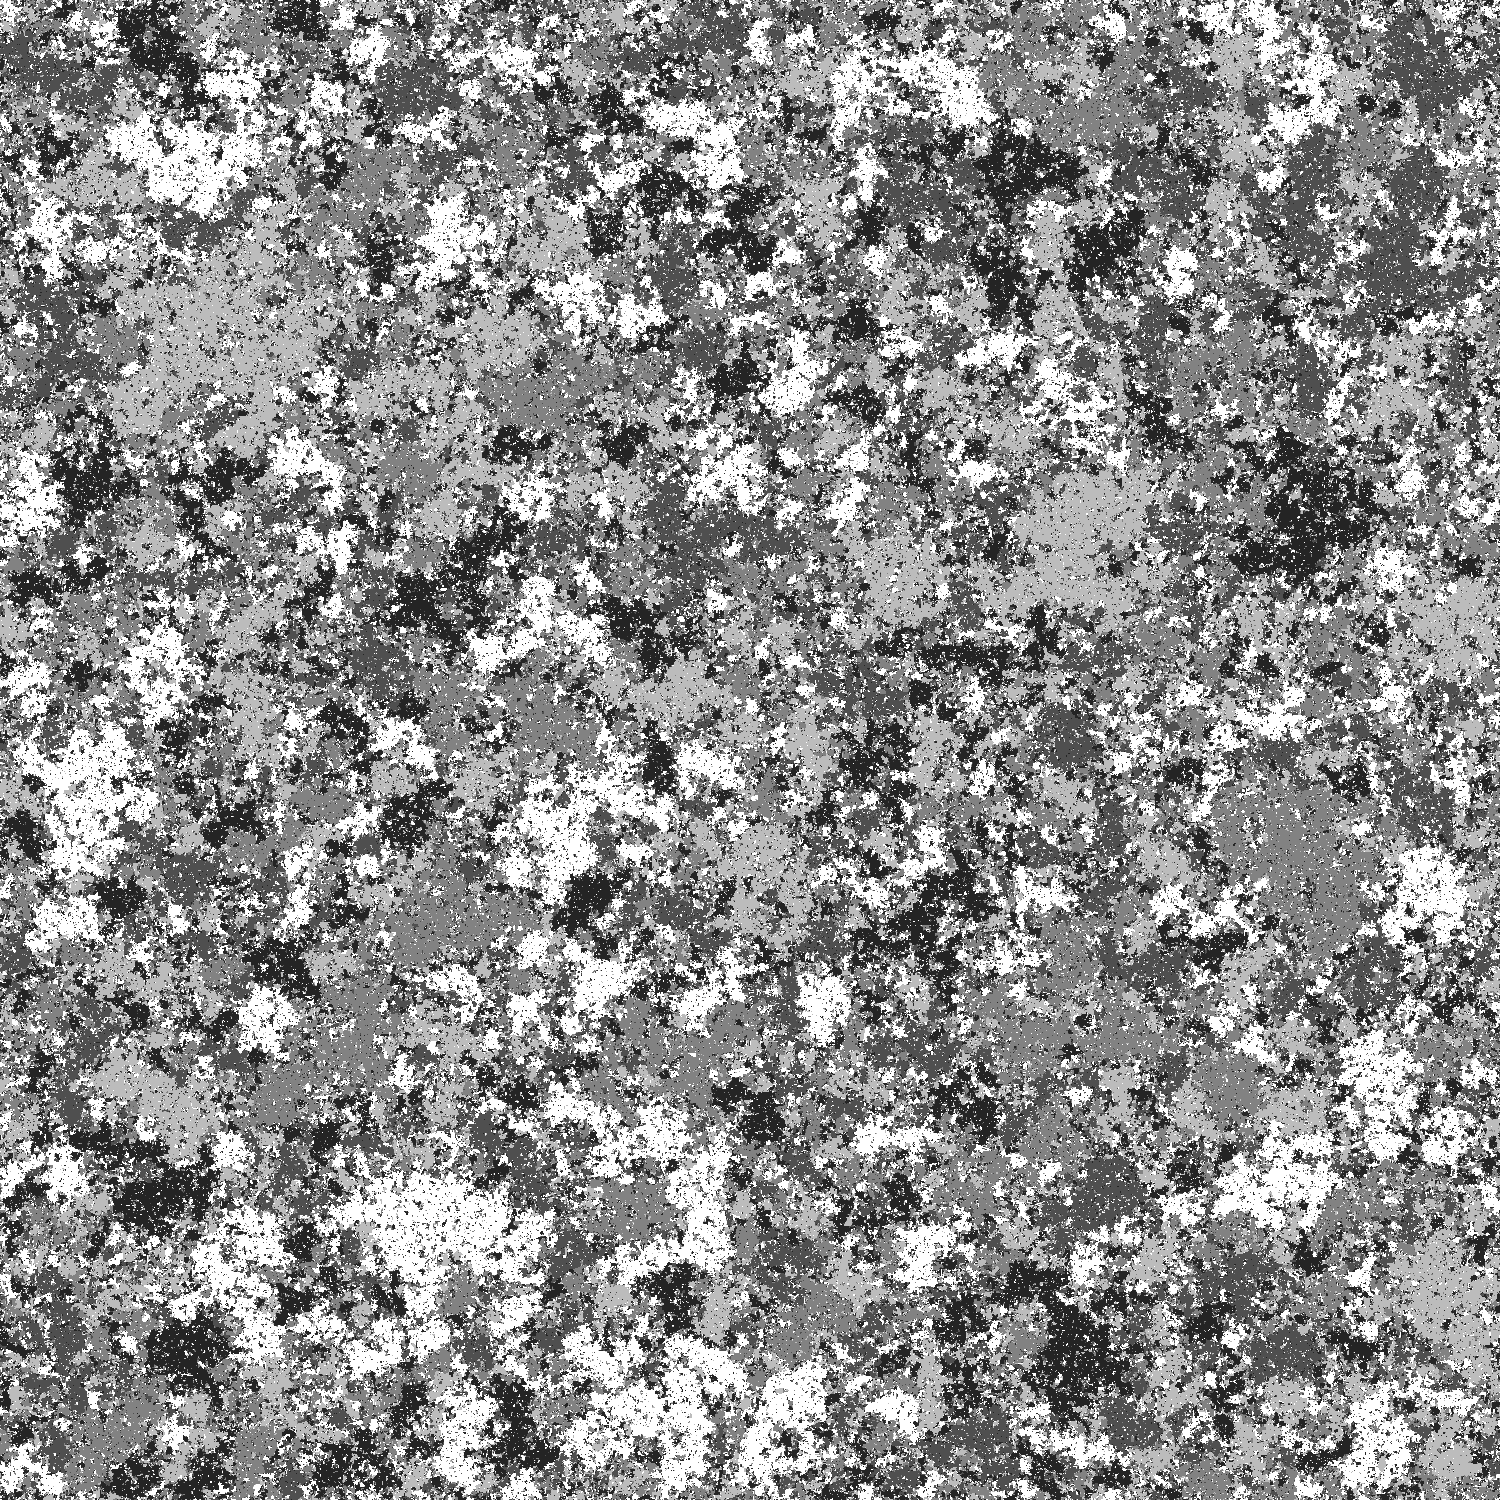
\includegraphics[width=.32\linewidth]{Classes1}}
\subfigure[Second map of $5$ classes]{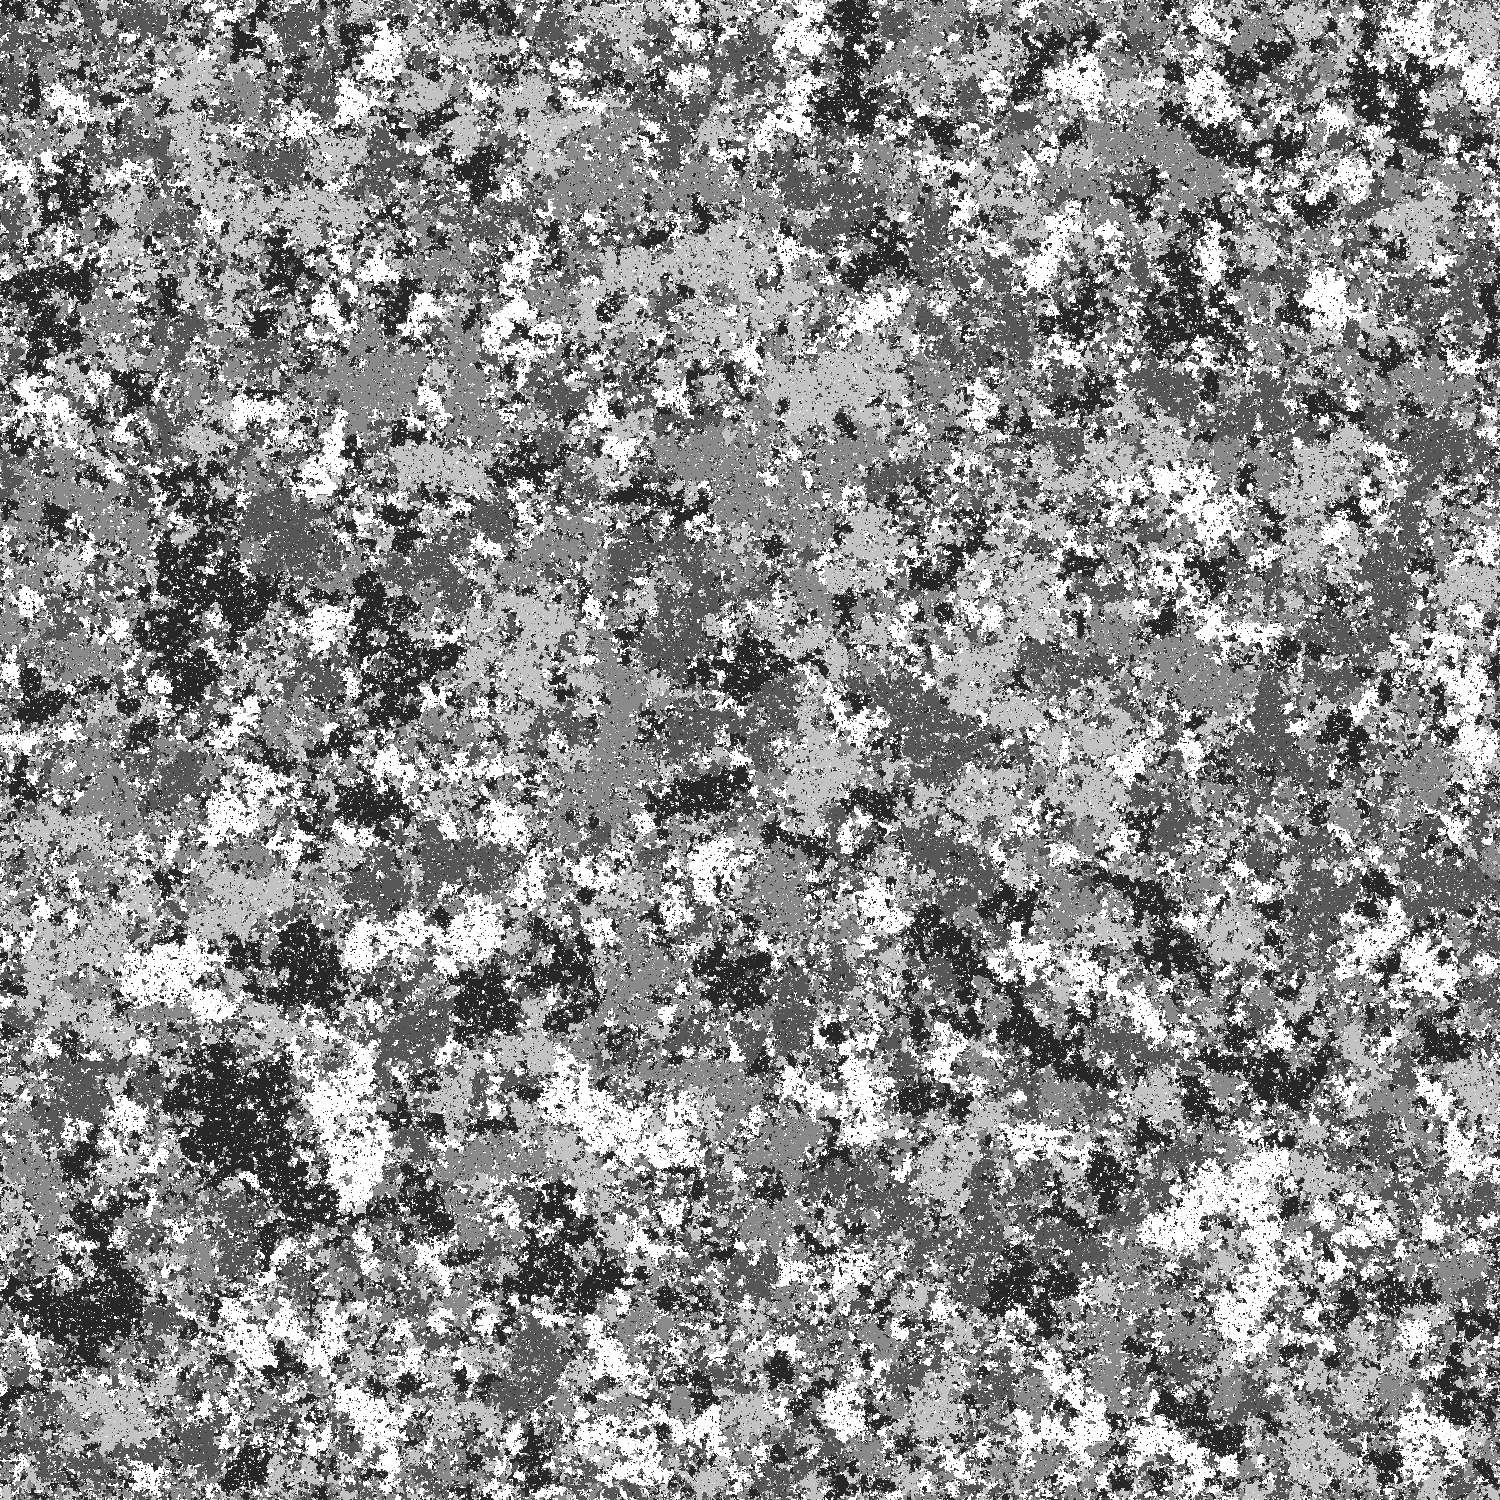
\includegraphics[width=.32\linewidth]{Classes2}}\\
\subfigure[Roads\label{image:Roads}]{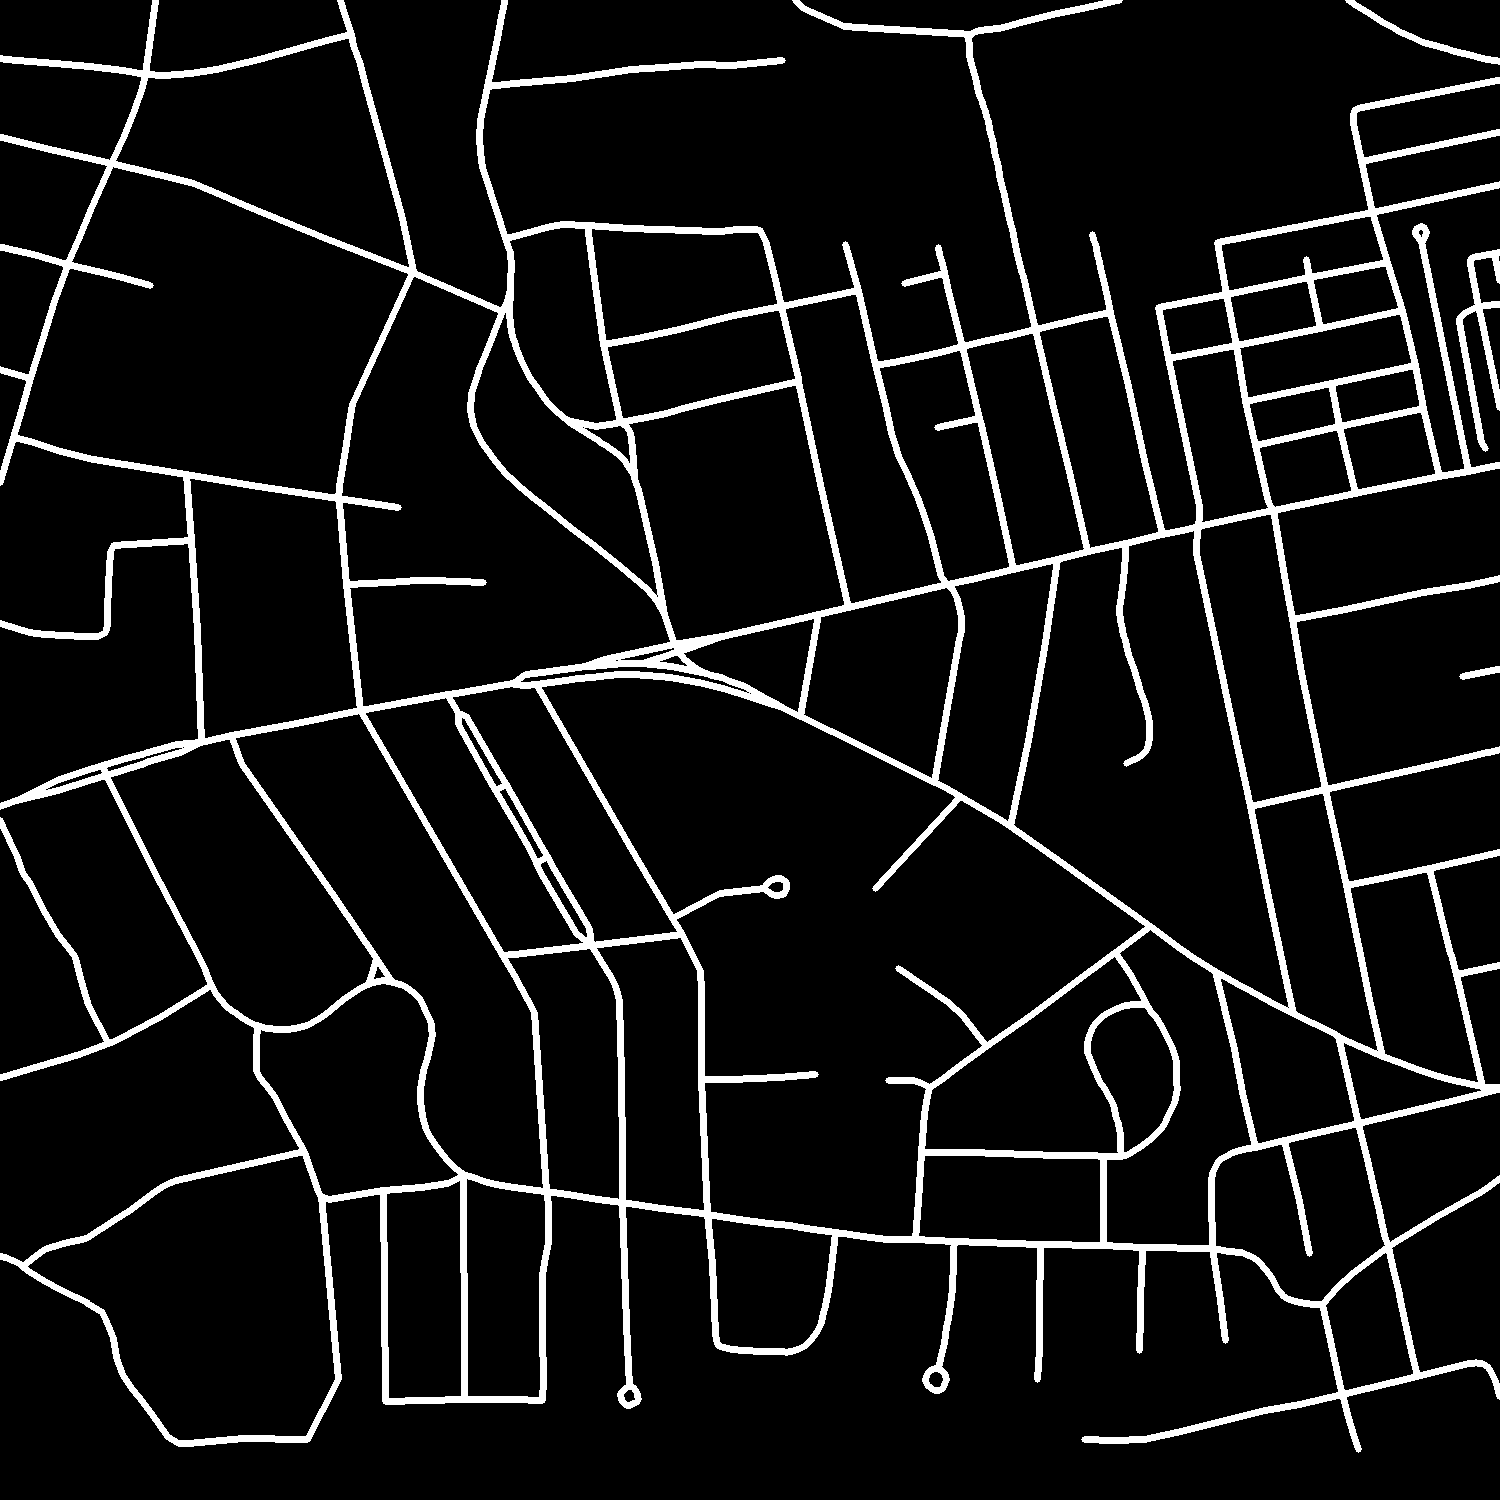
\includegraphics[width=.32\linewidth]{1052873515}}
\subfigure[First map with roads\label{image:M1Roads}]{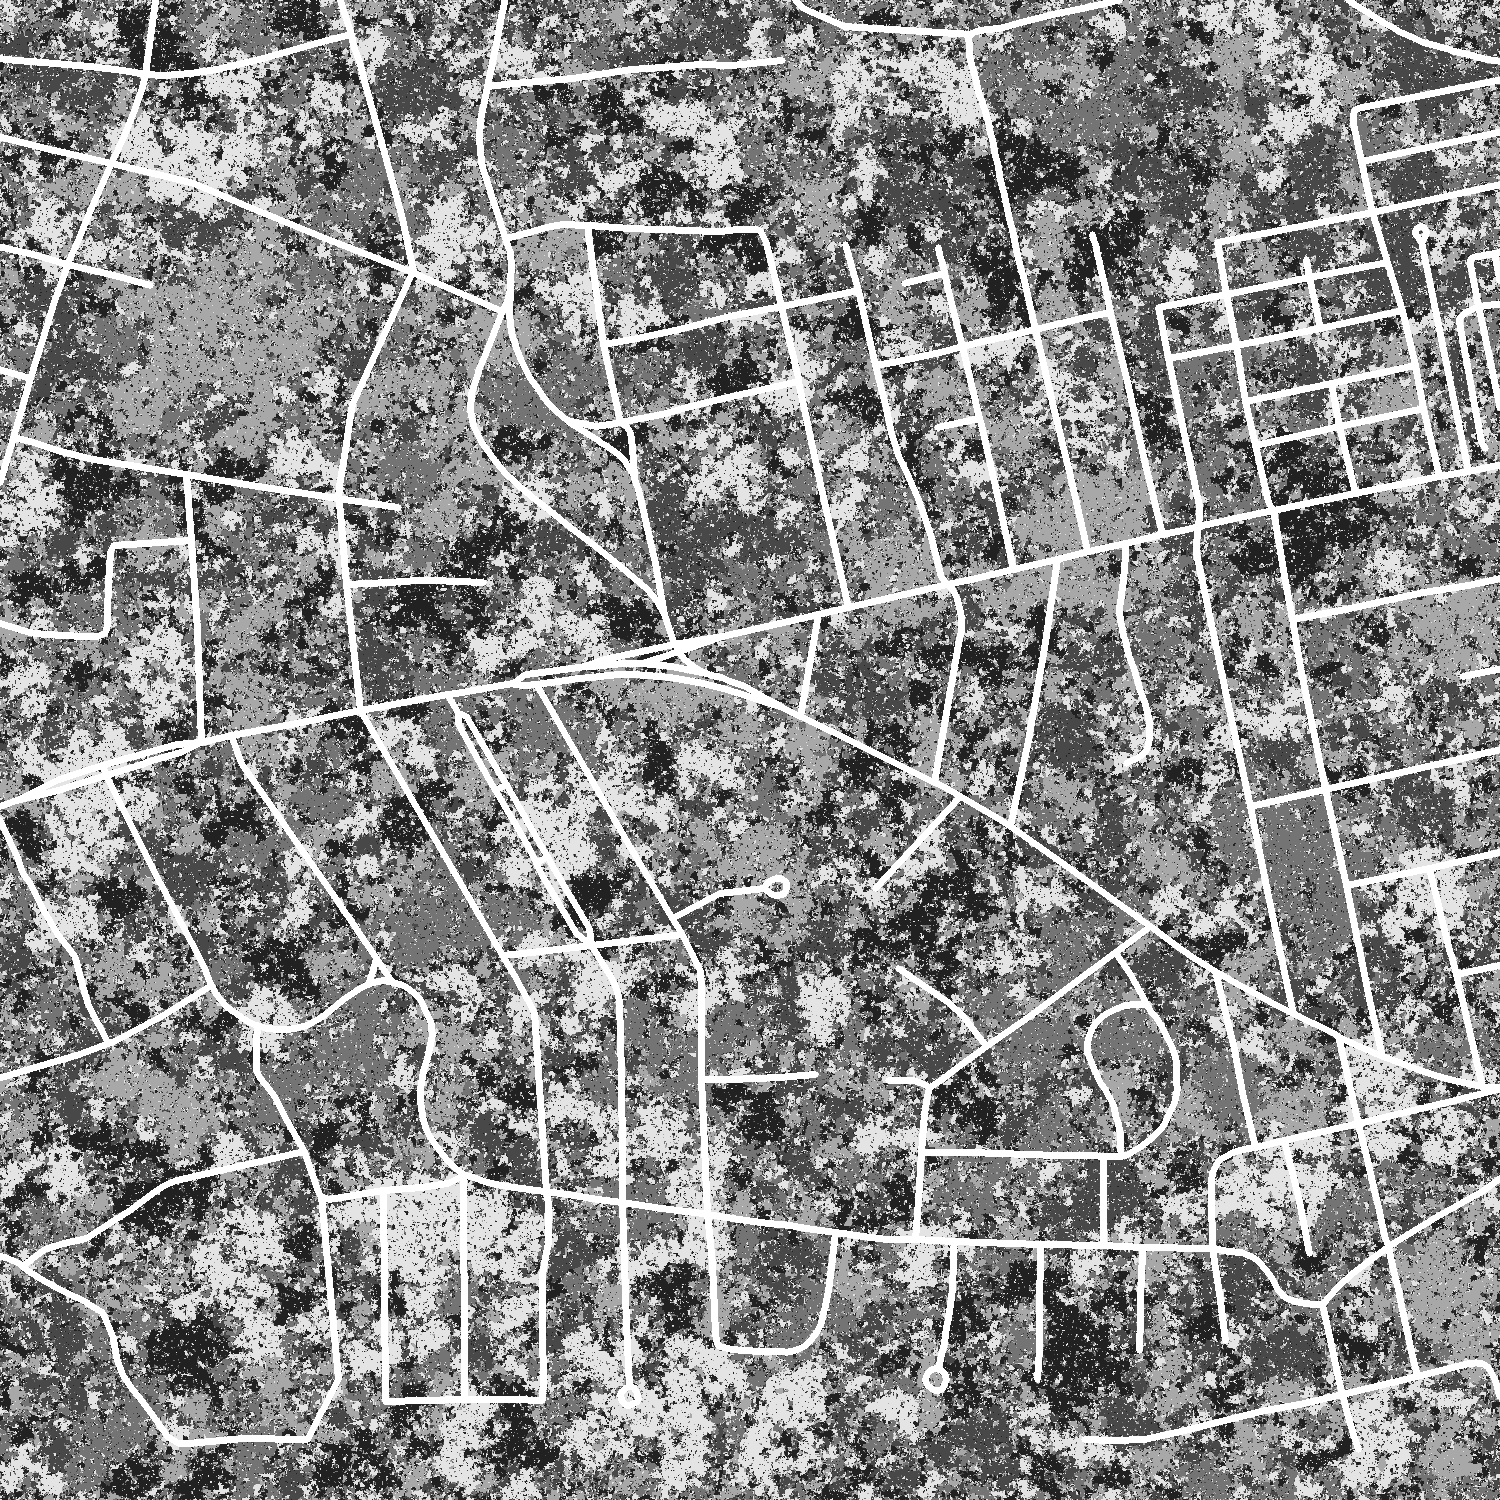
\includegraphics[width=.32\linewidth]{Class1Roads}}
\subfigure[Second map with roads\label{image:M2Roads}]{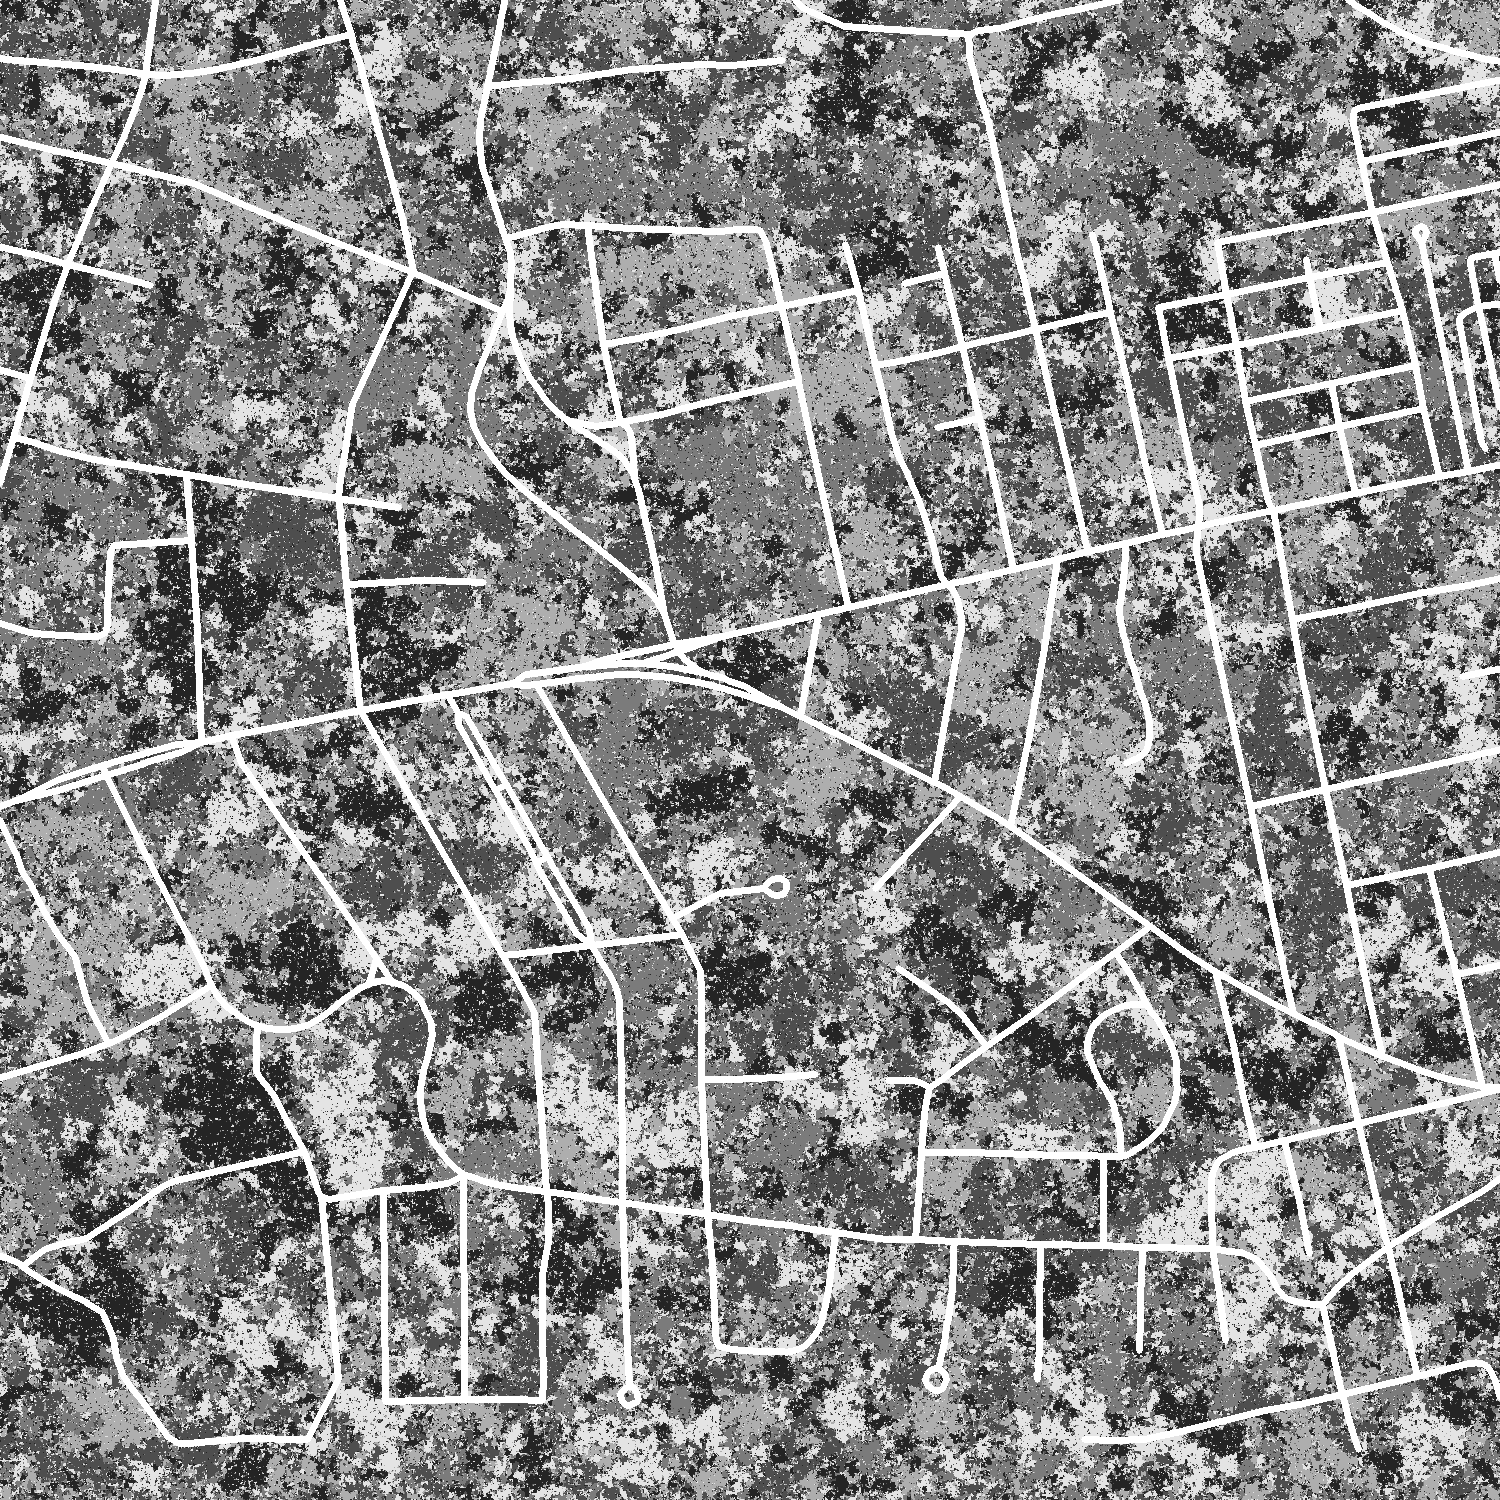
\includegraphics[width=.32\linewidth]{Class2Roads}}
\caption{Maps of classes}\label{fig:MapsClasses}
\end{figure*}

Since we are interested in simulating plausible SAR images, the data should obey the multiplicative model.
Without loss of generality, we consider intensity data with fully developed speckle, therefore, following Gamma distributions.

Each of the $k=1$ classes will have a different mean $\mu_i$, $1\leq i\leq k+1$ and the same number of looks $L$.
For the first set of classes and roads we chose $L=1$, and 
$\mu_1=40$,
$\mu_2=60$,
$\mu_3=80$,
$\mu_4=100$, 
$\mu_5=200$, and
$\mu_6=30$.
The second set of classes is transformed into SAR data using $L=3$, and 
$\mu_1=50$,
$\mu_2=100$,
$\mu_3=150$,
$\mu_4=200$, 
$\mu_5=500$, and
$\mu_6=10$.

Fig.~\ref{fig:Densities13} shows the densities used to model with one and three looks.

\begin{figure}
\centering
\subfigure[Densities for the single-look image\label{fig:Dens1Look}]{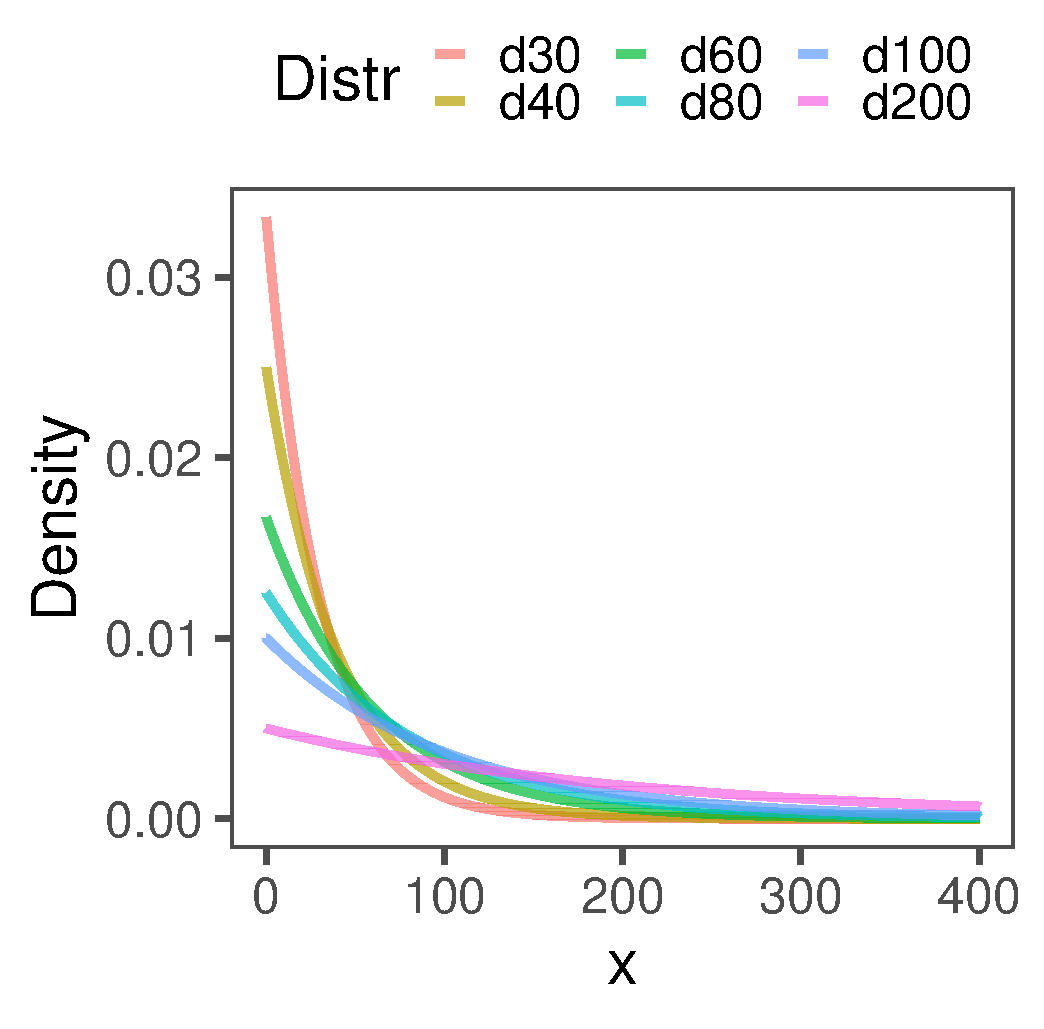
\includegraphics[width=\linewidth]{DensitiesSAR1}}
\subfigure[Densities for the three-look image\label{fig:Dens3Look}]{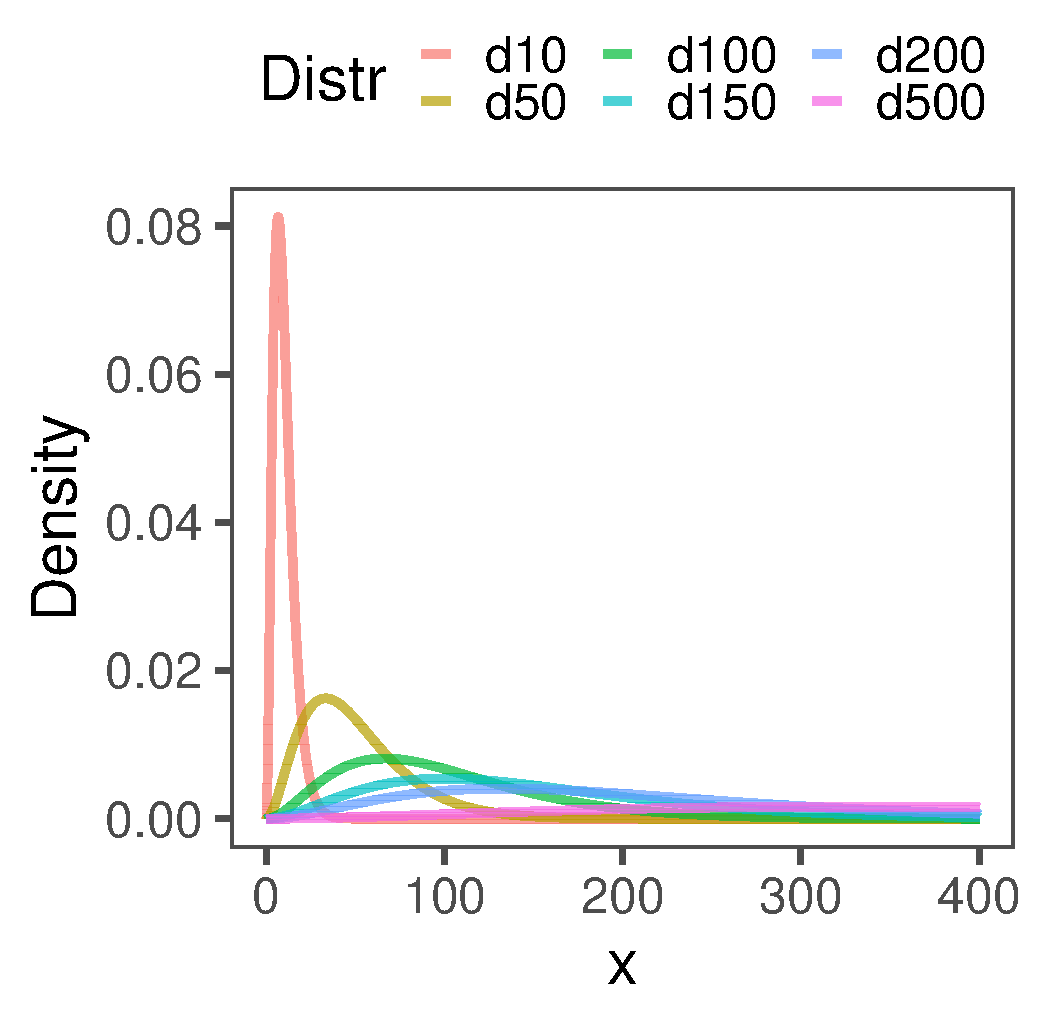
\includegraphics[width=\linewidth]{DensitiesSAR2}}
\caption{Densities for the single- and three-look images}\label{fig:Densities13}
\end{figure}

\begin{figure}[hbt]
\centering
\subfigure[Simulated SAR image, single look\label{image:SingleLook}]{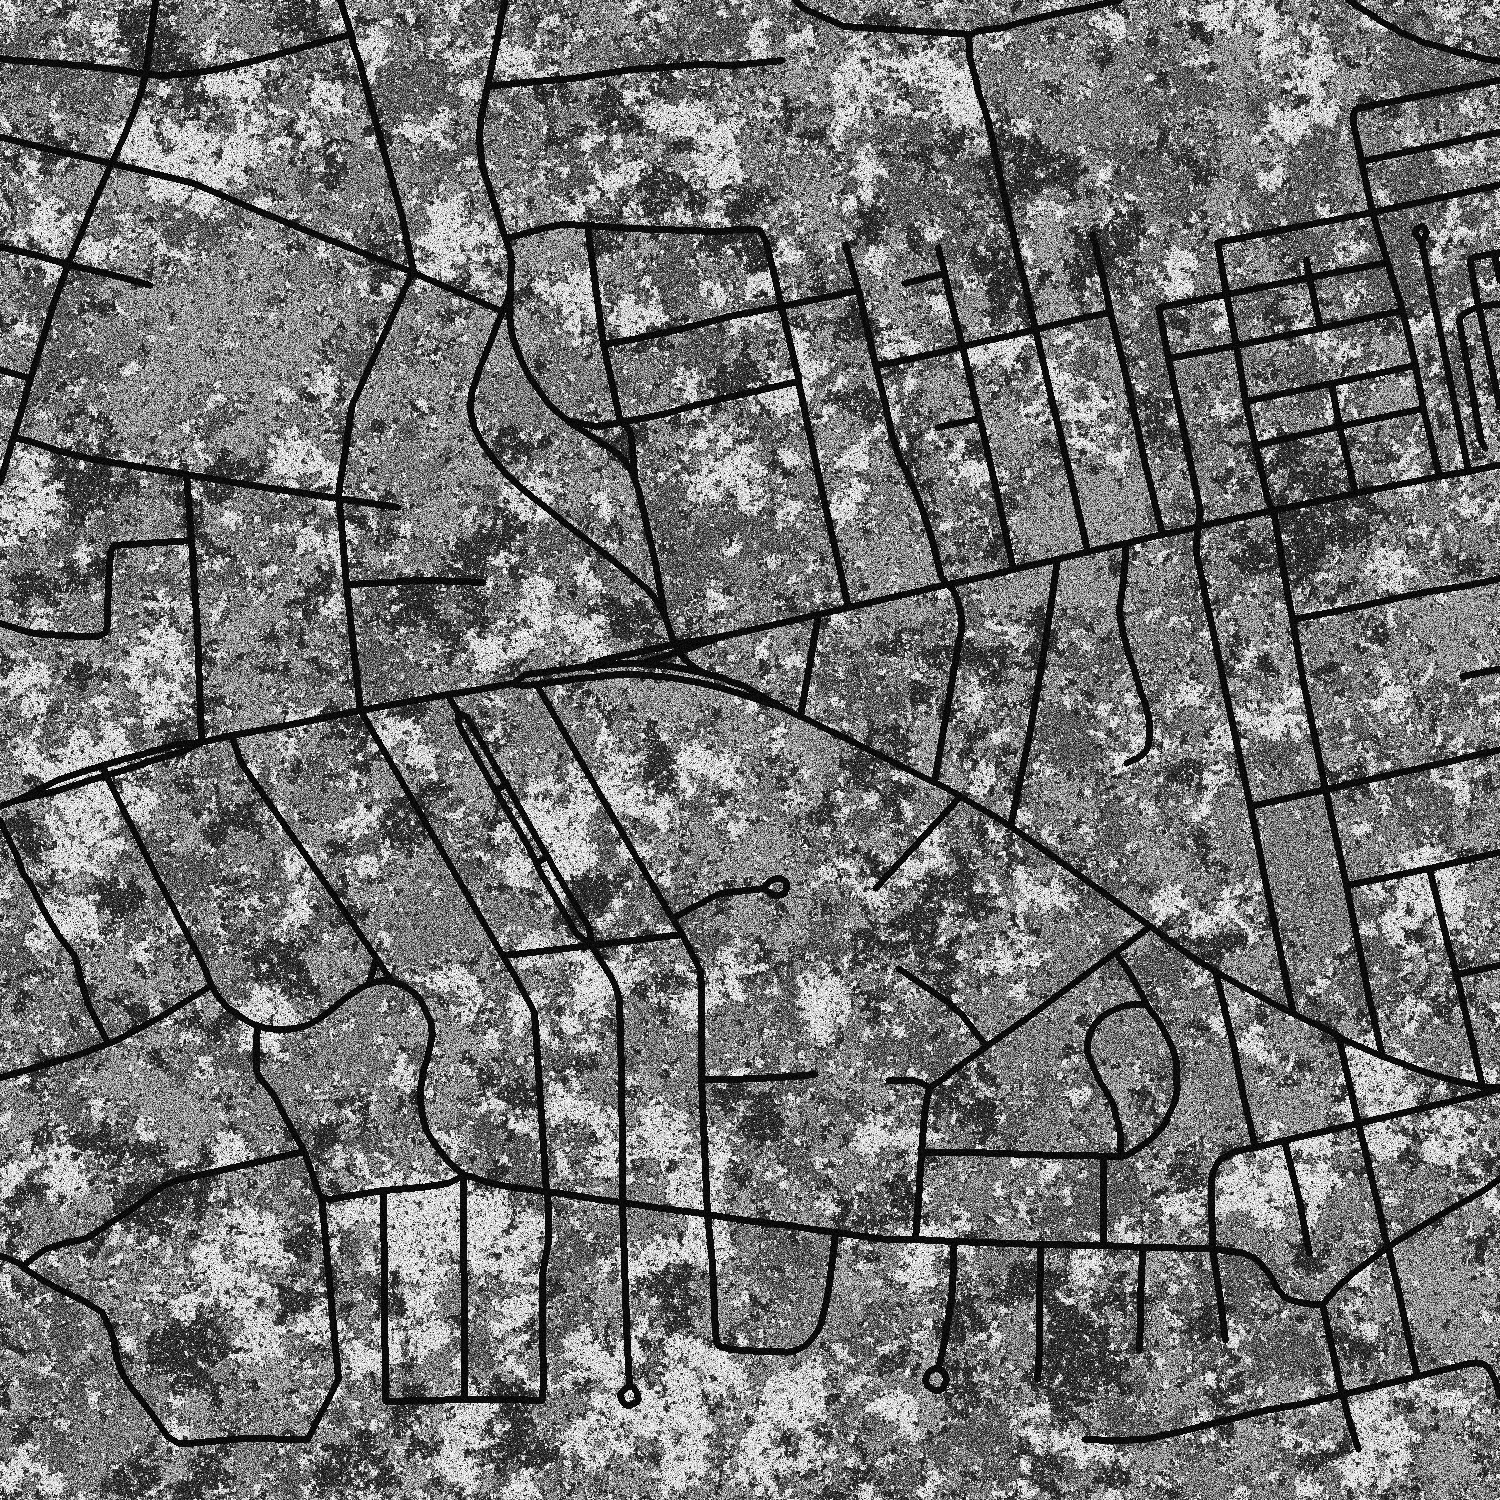
\includegraphics[width=\linewidth]{1look}}\\
\subfigure[Simulated SAR image, three looks\label{image:ThreeLooks}]{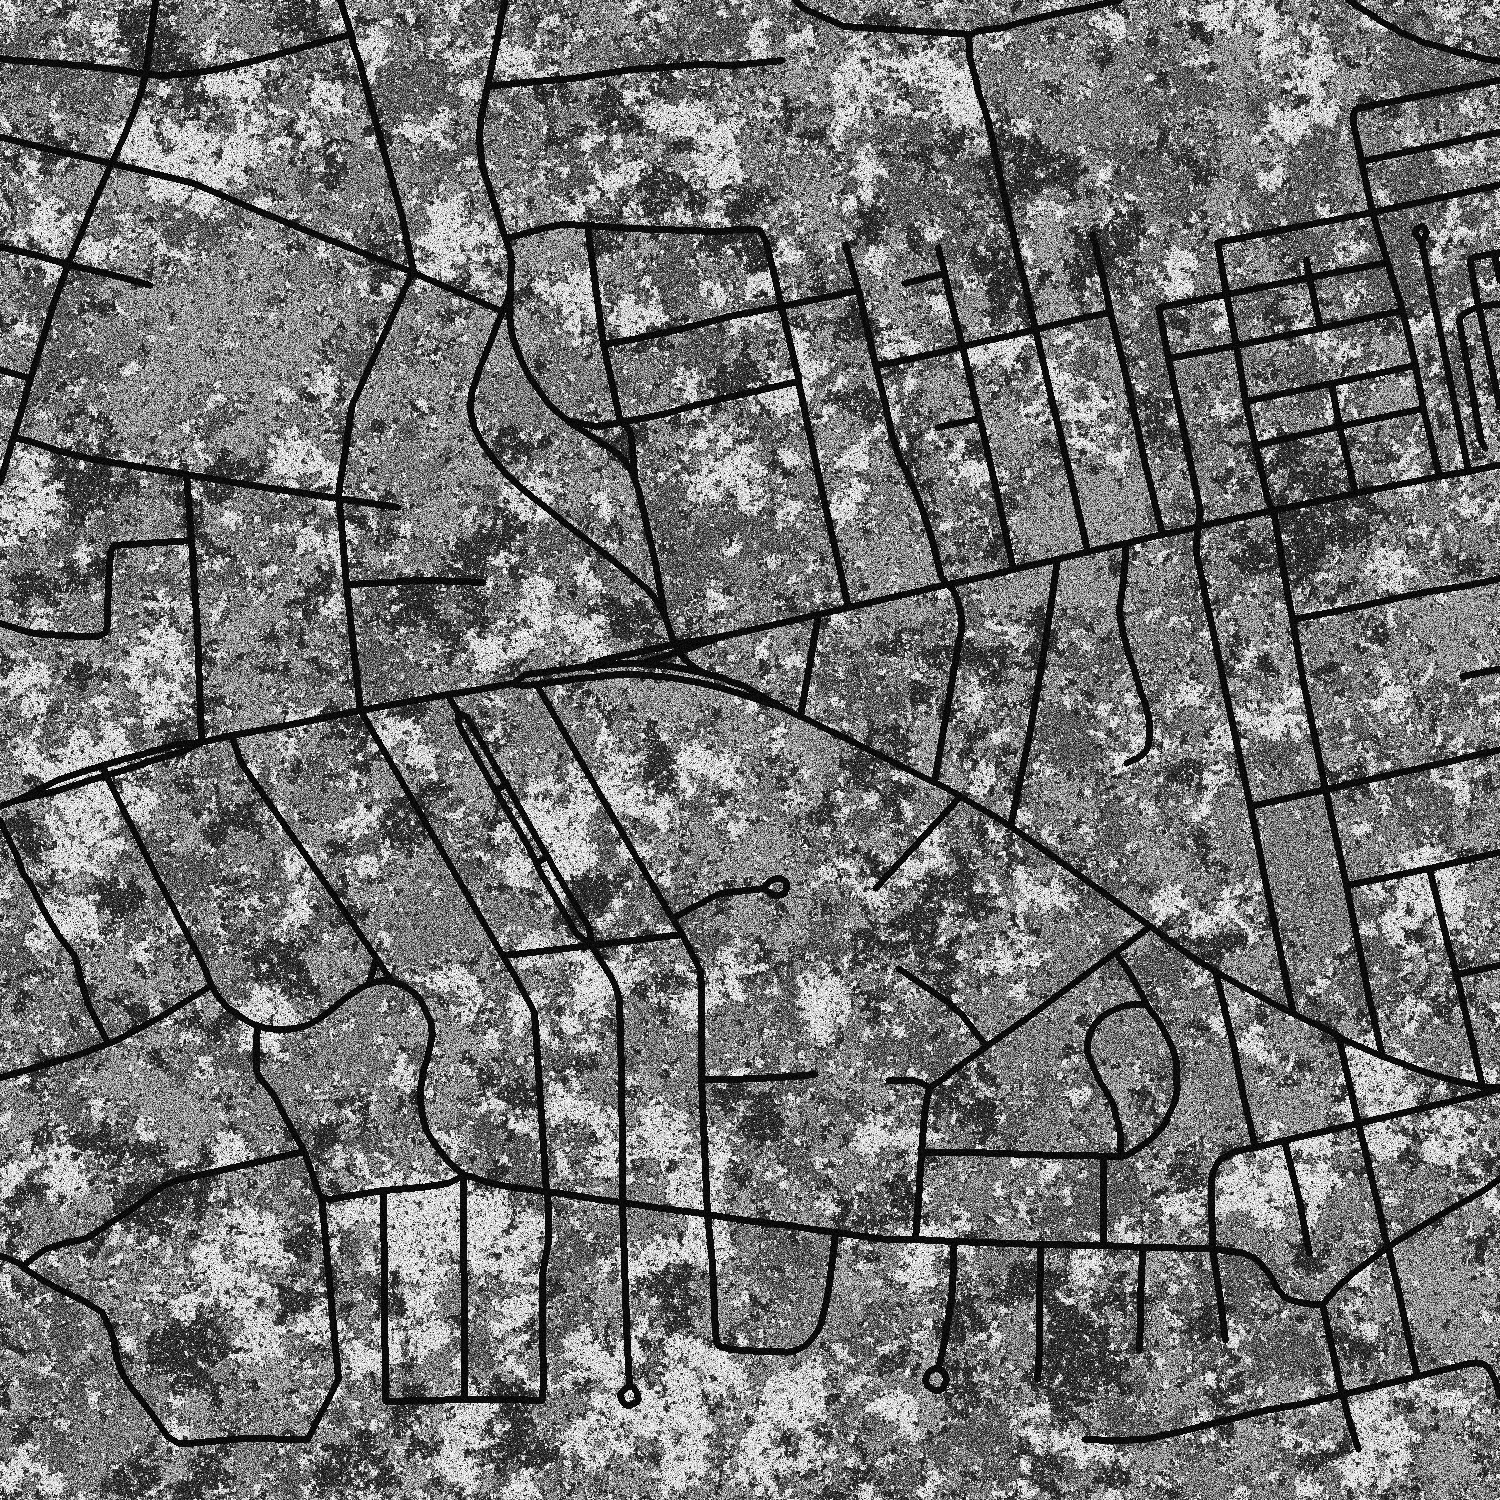
\includegraphics[width=\linewidth]{3looks}}
\caption{Results of the proposed simulation pipeline}\label{fig:Pipeline}
\end{figure}

This approach allows obtaining an arbitrary number of samples of SAR images $Z$ from scenes $X$ with roads $X'$ corrupted by speckle with specified distributions.

\appendix

\section{Computational Information}

We obtained the Potts model samples using 
\verb|R|~\cite{R}, and
the \verb|bayesImageS| library~\cite{ScalableBayesianInferencefortheInverseTemperatureofaHiddenPottsModel2018}.

\bibliographystyle{IEEEtran}
\bibliography{../Common/bibliography}

\end{document}
